\section{Solution design}
We started with a system design step.
Regarding this, we realized sequence diagrams
that describe the sequences of interaction between the simple
frontend and the microservice-based backend. These also take
into account the communications that happen among different
microservices that are involved in the same use case. One example
is the restaurant reservation use case that passes
through an authentication microservice and another microservice
that handles the restaurants’ data. Here we describe the microservices
that we designed and attach the corresponding sequence diagrams showing
the interactions among them.

\subsection{Microservices}

\subsubsection{User auth}

The user auth microservice exposes an interface for authentication needs of the
user. These are mainly related to login and registration via the frontend web app
and identity validation via the backend for operations that need authentication.
The main idea is to have an API that responds to requests, by operating on a
NoSQL database. The database contains information about the users: Name, Surname,
Email address, Password, and Session Tokens. The user registers into the system
and a new entry in the database is created. When a user logs in, a new session
is created by generating a unique token. This token is stored in the database
and sent to the frontend to be cached. The system is purely RESTful and thus
stateless. Every request is authenticated via the auth token.\\
The available operations are:
\begin{itemize}
    \item Login (Figure \ref{fig:user_login}): The client provides email and
    password (or token) and receives a session token if the user is registered.
    \item Registration (Figure \ref{fig:user_registration}): The client provides name,
    surname, email and password, and receives a session token after being registered
    in the database. The operation fails if a user with the same email already exists.
    \item Logout: The current login session is canceled.
    \item Token validation: The calling microservice (the one that needs a request to
    be authenticated) provides the email and session token of the user that initiated
    the operation and receives a validation or an error, depending on the validity of
    the token. This operation is shown in Figure \ref{fig:reserve}.
\end{itemize}

\begin{figure}
    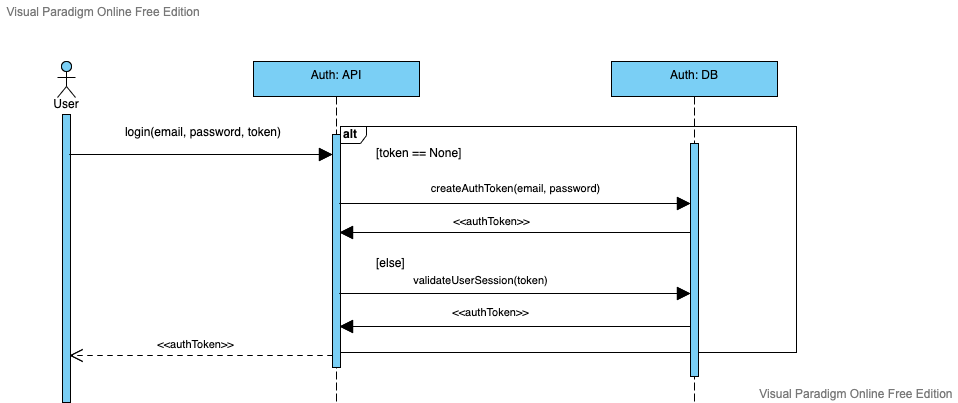
\includegraphics[width=17cm]{../docs/sequence/userAuth/auth.png}
    \caption{User login sequence diagram.}
    \label{fig:user_login}
\end{figure}

\begin{figure}
    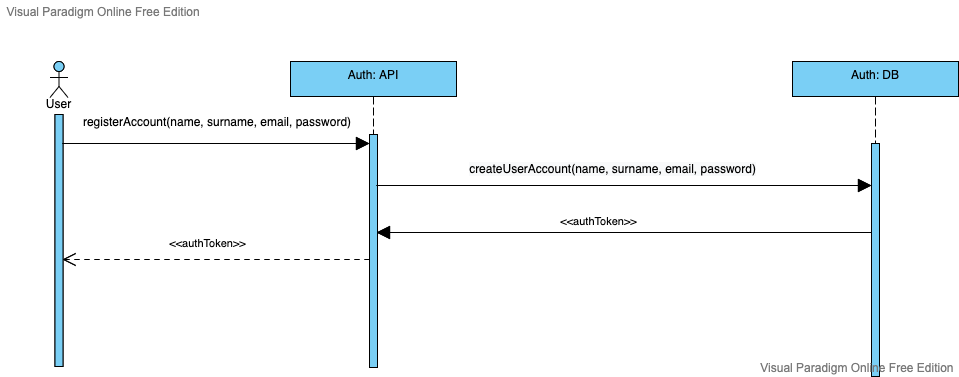
\includegraphics[width=\linewidth]{../docs/sequence/userRegistration/registerUser.png}
    \caption{User registration sequence diagram.}
    \label{fig:user_registration}
\end{figure}

\subsubsection{Restaurant auth}

The restaurant auth microservice exposes an interface for authentication needs of the
restaurant. It is very similar to the one of the user, but it is separated to better
divide contextes. In fact, the scalability needs of the two authentication services are
quite different. After the release of such a system, the increase in the number of users
is expected to be much more significant than the one of the number of registered
restaurants. This division guarantees individual scalability.
Also in this case there is an API that responds to requests, by operating on a
NoSQL database. The database contains authentication information about the restaurants:
Name, Email address, Password, and Session Tokens. The tokens work the same way they
do in the user auth module.\\
The available operations are:
\begin{itemize}
    \item Login (Figure \ref{fig:restaurant_login}): The client provides email and
    password (or token) and receives a session token if the user is registered.
    \item Logout: The current login session is canceled.
    \item Token validation: The calling microservice (the one that needs a request to
    be authenticated) provides the email and session token of the restaurant that initiated
    the operation and receives a validation or an error, depending on the validity of
    the token. This operation is shown in Figure \ref{fig:manage_booking}.
\end{itemize}

\begin{figure}[h]
    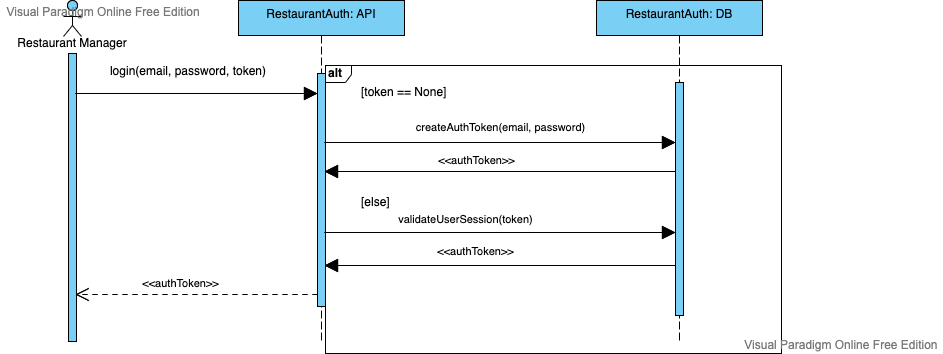
\includegraphics[width=\linewidth]{../docs/sequence/restaurantAuth/restaurantAuth.png}
    \caption{Restaurant login sequence diagram.}
    \label{fig:restaurant_login}
\end{figure}

\subsubsection{Restaurant data}

The Restaurant data microservice exposes an interface to search among different restaurants. After the log-in step, it is possible to search and select a restaurant in order to book it. \\
The search service operates on a NoSQL database containing data about the restaurant (name, address, email, rating, menu). Each restaurant is stored as a JSON object. The user can query the database through the service RESTful API. The sequence diagram is shown in Figure \ref{fig:restaurant_search}. \\
After the user has selected a restaurant, its unique ID is passed to the booking microservice. Disentangling the search service form the booking service allow us to have separated databases and thus to distribute the workload better. Indeed, this way individual scalability is assured: a user can search among all restaurants, but can book only one at a time. This consideration leads to the necessity to have decoupled services. \\
There is on possible operation to perform:

\begin{itemize}
    \item Search: the client provides a search string and receives a list of restaurants satisfying the search criteria;
\end{itemize}

\begin{figure}[h]
    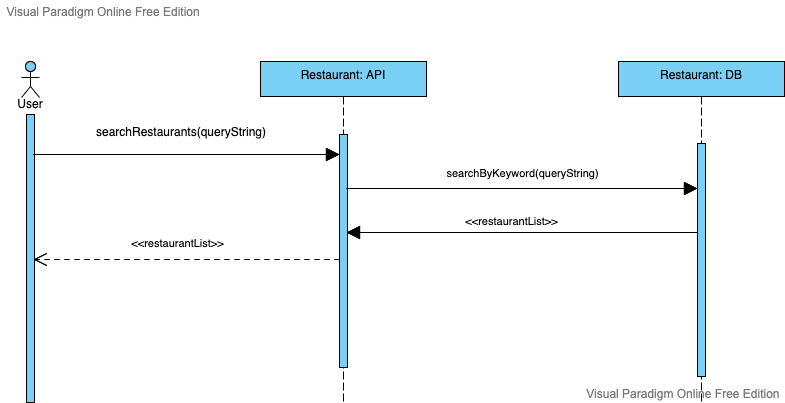
\includegraphics[width=\linewidth]{../docs/sequence/search/search.png}
    \caption{Restaurant search sequence diagram.}
    \label{fig:restaurant_search}
\end{figure}

\subsubsection{Booking}

This microservice offers all the functionalities that are needed to deal with the reservation of the tables in the restaurants. These functionalities can be used both from standard users and restaurant accounts, depending on the specific needs trough a REST API. More in detail users can send a request of table reservation to a specific restaurant, and this last can accept or deny this request. The service also have to offers other methods to retrieve the list of the reservations of a given user/restaurant. \\
This is one of the most important part of our whole application and also one of the most complex. To successfully complete all the task, this service has to communicate with \textit{ restaurant and user auth microservices } to validate the session tokens before commit all the operations.
As the others, this service relies on a NoSQL database to store reservations records. For each reservation a unique code identifier is generated and also the email of both restaurant and user are saved as contact info and also to link the requests with the accounts. The reservation also require these other fields: \textit{"date", "service", "time", "seats", "notes", "status"}. When a request is sent, its first status is set to \textit{"pending}". The tree possible status that a request can assume and that the microservice allow are: \textit{"pending","accepted","refused}".
So, in detail, the available operations are:

\begin{itemize}
    \item Reserve (Figure \ref{fig:reserve}): A standard user  send a request of a reservation to a specific restaurant providing all the required fields plus its session token that has to be validated in order to successfully complete the request. 
    \item Change status  (Figure \ref{fig:manage_booking}): The restaurant wants to change the status of a request, accepting or denying the reservation. To complete this operation the restaurant has to sent the reservation\_id, its email and the auth token to do other checks, and the new status. The operation can fail if the new status is not into the set of the allowed status, if the token is not valid, or if the reservation is not associated to that restaurant.
    \item Retrieve: Each restaurant or standard user has the possibility to retrieve all its reservation record.
    
\end{itemize}


\begin{figure}[h]
    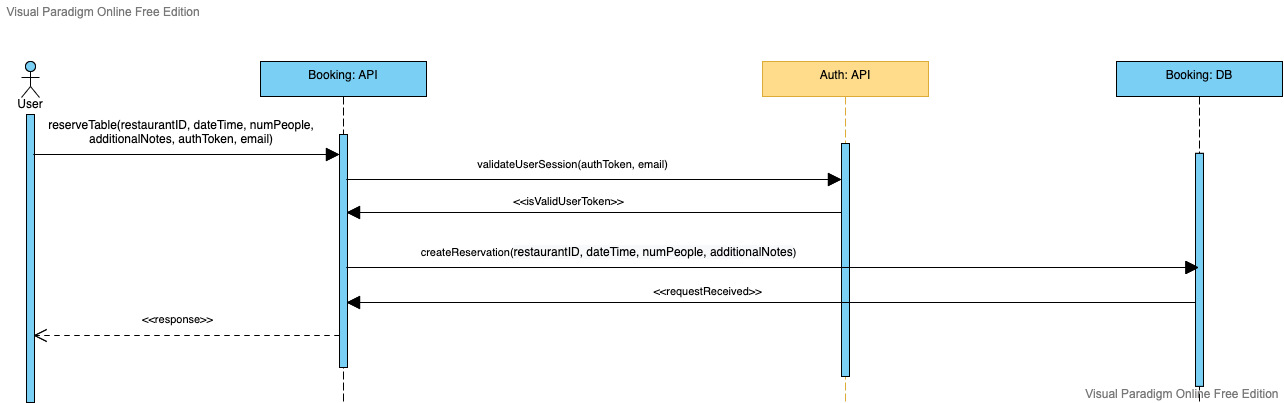
\includegraphics[width=\linewidth]{../docs/sequence/booking/reserve.png}
    \caption{Reservation sequence diagram.}
    \label{fig:reserve}
\end{figure}

\begin{figure}[h]
    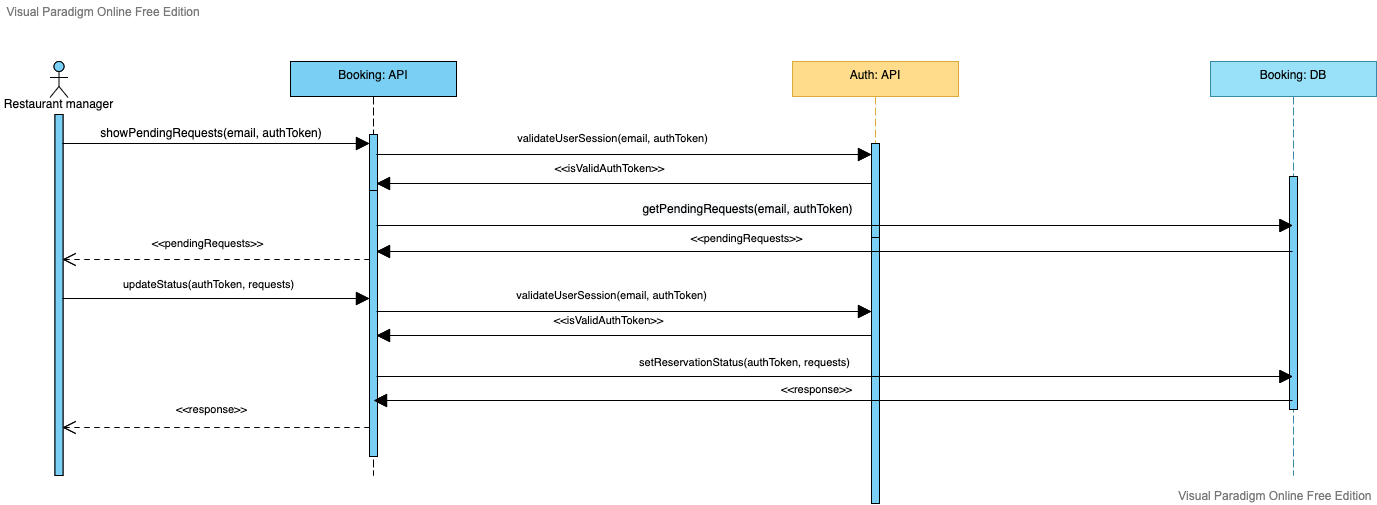
\includegraphics[width=\linewidth]{../docs/sequence/manageBooking/manageBooking.png}
    \caption{Booking management sequence diagram.}
    \label{fig:manage_booking}
\end{figure}

\subsection{Scalability, Availability and Continuous Deployment}

By structuring the system into many microservices, there is the possibility
to scale the single microservices indipendently. This is useful since the
microservices may receive different loads of incoming traffic and this
way there is more control over which component should be scaled. In a real world scenario, of course, standard users are expected to be much more respect restaurant account and we want to have an high level degree of elasticity.
Another important features is availability and fault isolation. If a part of the system goes down (e.g. restaurant data service), the rest of the application can still live and allow other operations (e.g. the reservation service).
The last important quality of this system is the simplicity, it is composed by small microservices that can be developed quickly, and that can also be upgraded in a fast way. We can explore the benefits of continuous development, in fact we can also decide to add other microservices in the future, as one for the reviews management, one for the mail notifications, and so on.
